% !TeX encoding = UTF-8
% 
% 作者: @yongjian.li 澳門科技大學-畢業論文latex模板-2023
% GitHub.project: https://github.com/iihciyekub/MUST-Thesis
% GitHub.io: https://iihciyekub.github.io/must-thesis-tools/#/
% Overleaf(read): https://www.overleaf.com/read/mjzpcxztzqzv
% 
% 最後更新: 2023-04-13
% 更新內容: 
% 1. 增加 bib2bbl 工具, 將bib 直接轉換成符合must 關於畢業論文文獻排版要求的格式,
%   - 本项目目录下 .tool/bib2bbl.html (本地運行)
%   - https://pychat.online/bib2bbl (网址2024/03/01 之前有傚)
%   - chrom 插件,內測中未發佈, 可從 github 下載自行安裝 https://github.com/iihciyekub/must-thesis-tools 


\documentclass[
    添加扉頁=是,
    添加原創聲明頁=不,
    添加校徽水印=是,
    奇偶頁邊距對稱=不,
    參考文獻頂格=是,
]{.def/must}



% 論文基本信息,必填不能刪除
\def\shool              {澳門科技大學}
\def\cntitle            {XXX 銀行(澳門分行)與 XXX 銀行合並之研究}
\def\entitle            {The Study of XXX Bank (Macau Branch) Merged the XXX Bank in Macao}
\def\Name               {XXX}% 名稱
\def\StudentNo          {1809853G-BM30-0053}% 學號
\def\Faculty 	        {XXX 學院}% 所在學院
\def\Program 	        {XXXX}% 課程名稱
\def\Major              {XXXX}% 專業名稱
\def\Supervisor	        {XXXX}% 指導老師
\def\DateofWriting		{\datea\today}% 設置論文寫作完成時間
\def\DateofDeclaration	{\dateb\today}% 設置論文原創聲明時間
\def\DateofSignature	{2023/06/30}% 設置簽署論文原創聲明的時間
\def\PublicAfterYears   {0}% 設置論文幾年後公開



 
\begin{document}
\begin{abstract@cn}{關鍵字1、關鍵字1、關鍵字1、關鍵字1}
本研究採用2009 年至2014 年首度上市的公司279 家為研究
樣本,檢驗公司治理與財務績傚之關聯性。利用樣本公司上市時
的公司治理變數,檢驗公司治理對上市後的會計績傚影響與上市
後30 天的市場報酧,再進而依據過去文獻對公司治理變數的論
述,以單一指標衡量,依研究對象中位數區分公司治理程度,以
及公司治理變數給予不同分數,驗證對財務績傚之影響,並比較
「有價證券上市審查準則」強化公司治理制度前後之上市公司,
在公司治理與財務績傚上是否有差異。透過相關分析、T 檢定、
迴歸分析,檢驗三大研究假說,實證結果獲得以下主要結論:
本研究採用2009 年至2014 年首度上市的公司279 家為研究
樣本,檢驗公司治理與財務績傚之關聯性。利用樣本公司上市時
的公司治理變數,檢驗公司治理對上市後的會計績傚影響與上市
後30 天的市場報酧,再進而依據過去文獻對公司治理變數的論
述,以單一指標衡量,依研究對象中位數區分公司治理程度,以
及公司治理變數給予不同分數,驗證對財務績傚之影響,並比較
「有價證券上市審查準則」強化公司治理制度前後之上市公司,
在公司治理與財務績傚上是否有差異。透過相關分析、T 檢定、
迴歸分析,檢驗三大研究假說,實證結果獲得以下主要結論:
本研究採用2009 年至2014 年首度上市的公司279 家為研究
樣本,檢驗公司治理與財務績傚之關聯性。利用樣本公司上市時
的公司治理變數,檢驗公司治理對上市後的會計績傚影響與上市
後30 天的市場報酧,再進而依據過去文獻對公司治理變數的論
述,以單一指標衡量,依研究對象中位數區分公司治理程度,以
及公司治理變數給予不同分數,驗證對財務績傚之影響,並比較
「有價證券上市審查準則」強化公司治理制度前後之上市公司,
在公司治理與財務績傚上是否有差異。透過相關分析、T 檢定、
迴歸分析,檢驗三大研究假說,實證結果獲得以下主要結論:
本研究採用2009 年至2014 年首度上市的公司279 家為研究
樣本,檢驗公司治理與財務績傚之關聯性。利用樣本公司上市時
的公司治理變數,檢驗公司治理對上市後的會計績傚影響與上市
後30 天的市場報酧,再進而依據過去文獻對公司治理變數的論
述,以單一指標衡量,依研究對象中位數區分公司治理程度,以
及公司治理變數給予不同分數,驗證對財務績傚之影響,並比較
「有價證券上市審查準則」強化公司治理制度前後之上市公司,
在公司治理與財務績傚上是否有差異。透過相關分析、T 檢定、
迴歸分析,檢驗三大研究假說,實證結果獲得以下主要結論:
\end{abstract@cn}



\begin{abstract@en}{keyword1、keyword1、keyword1、keyword1、}
This research used 279 companies established between 2009 and 2014 as the
sample, examining the relationship between corporate governance and financial
performance. Corporate governance variable during the time when company
gets started is used to examine the effect of corporate governance on accounting
effectiveness after the company has been on the market, as well as the effect on
the return rate during the first 30 days of the company’s opening. Further
analysis from literature review on corporate governance, using single
measurement, is according to the median of the level of corporate governance
and the rating of corporate governance variable, to cross examine its effect on
financial performance. Also, a comparison of the effect on strengthening
corporate governance using “Stock Exchange Listing Standards” before and
after the company was listed on the stock market on corporate governance and
financial performance. Correlation, T-test, and Regression analysis were used to
examine three hypotheses. Findings include: 
\begin{enumerate}[leftmargin=1.2 em,label=\arabic*) ]
    \item  Company characteristics
High Tech industry has better corporate governance mechanism than traditional
industries.
    \item  Characteristic of corporate governance level
High corporate governance companies have better accounting effectiveness and
market performance.
    \item  Correlation between economic cycle and industry type v.s. corporate
 governance and management effectiveness
Industry characteristics will reinforce the impact of corporate governance level
towards accounting effectiveness; whereas economic cycle will reinforce the
impact of corporate governance level toward market effectiveness.
    \item  In a time of recession, corporate governance showed positive effect on
market effectiveness.
    \item  Corporate governance has a positive correlation with accounting
effectiveness when there were fewer diversified investors; with the
exception of high tech industry, which shows positive correlation between
corporate governance level and accounting effectiveness when there were
more diversified investors.
    \item  Companies participated in strengthening corporate governance since the
policy was enforced showed positive relationship with management
effectiveness.
    \item  Better corporate governance and management effectiveness since the
legislation was enforced.
    \item  Corporate governance is stronger among the high tech industry. 
\end{enumerate}
This research used 279 companies established between 2009 and 2014 as the
sample, examining the relationship between corporate governance and financial
performance. Corporate governance variable during the time when company
gets started is used to examine the effect of corporate governance on accounting
effectiveness after the company has been on the market, as well as the effect on
the return rate during the first 30 days of the company’s opening. Further
analysis from literature review on corporate governance, using single
measurement, is according to the median of the level of corporate governance
and the rating of corporate governance variable, to cross examine its effect on
financial performance. Also, a comparison of the effect on strengthening
corporate governance using “Stock Exchange Listing Standards” before and
after the company was listed on the stock market on corporate governance and
financial performance. Correlation, T-test, and Regression analysis were used to
examine three hypotheses. Findings include:
\end{abstract@en}


% 添加目錄 
\addtableofcontents



\chapter{緒論}





\section{研究動機與目的}
\subsection{研究動機}
\par 美國學者對公司治理的討論可追溯自1930 年代,Berle \&
Means(1932)指出,美國企業存在著股權分散的必要性,因為隨著企
業規模不斷的擴大,使得多數的中大型公司皆需將經營權與所有權
加以分離來經營,以期達到專業化的目的。
\par 有系統地討論此一問題者為Jensen,在1988 年Jensen 首度有系統地
收錄以公司治理為主題的文章(Weston, Siu \& Johnson; 2002)。

\noindent 公式:式子置中,編號靠右,如


\begin{equation}
V_0=X_0(1-T)(1-b) \sum_{t=1}^n \frac{(1+g)^t}{(1+k)^t}+\frac{X_0(1-T)(1-g)^{n+1}}{k(1+k)^n}
\end{equation}


\par 美國學者對公司治理的討論可追溯自1930 年代,Berle \&
Means(1932)指出,美國企業存在著股權分散的必要性,因為隨著企
業規模不斷的擴大,使得多數的中大型公司皆需將經營權與所有權
加以分離來經營,以期達到專業化的目的。
$V_0=X_0(1-T)(1-b) \sum_{t=1}^n \frac{(1+g)^t}{(1+k)^t}+\frac{X_0(1-T)(1-g)^{n+1}}{k(1+k)^n}$ 
有系統地討論此一問題者為Jensen,在1988 年Jensen 首度有系統地
收錄以公司治理為主題的文章(Weston, Siu \& Johnson; 2002)。
\begin{enumerate}
\item 第一個枚舉\\ 第一個枚舉換行
\item 第二個枚舉 
\item 第三個枚舉 
\end{enumerate}

% 添加表格
\begin{table}[htbp]
    \centering
    \caption{讀取 csv 數據}
    \label{tab:mytable}
    \csvautobooktabular{data.csv} 
\end{table}




\begin{sidewaystable}[!htp]
	\caption{示例旋轉長表} 
	\centering
	\setlength{\tabcolsep}{10mm}
	\begin{tabular}[l]{@{}lcccccc}		
	\toprule		
	Class$^{\rm a}$ & $\gamma_1$ & $\gamma_2$$^{\rm b}$& $\langle \gamma \rangle$& $G$ & $|{ f}|$ & $\theta _{c}$ \\		
	\midrule	
        BL Lacs &5 & 36 & 7 & $-4.0$ & $1.0\times 10^{-2}$ & 10$^\circ$ \\		
        FSRQs & 5 & 40 & 11 & $-2.3$ & $0.5\times 10^{-2}$ & 14$^\circ$ \\	
        FSRQs & 5 & 40 & 11 & $-2.3$ & $0.5\times 10^{-2}$ & 14$^\circ$ \\	
        FSRQs & 5 & 40 & 11 & $-2.3$ & $0.5\times 10^{-2}$ & 14$^\circ$ \\	
        FSRQs & 5 & 40 & 11 & $-2.3$ & $0.5\times 10^{-2}$ & 14$^\circ$ \\	
        FSRQs & 5 & 40 & 11 & $-2.3$ & $0.5\times 10^{-2}$ & 14$^\circ$ \\	
        FSRQs & 5 & 40 & 11 & $-2.3$ & $0.5\times 10^{-2}$ & 14$^\circ$ \\	
        BL Lacs &5 & 36 & 7 & $-4.0$ & $1.0\times 10^{-2}$ & 10$^\circ$ \\		
        FSRQs & 5 & 40 & 11 & $-2.3$ & $0.5\times 10^{-2}$ & 14$^\circ$ \\	
        FSRQs & 5 & 40 & 11 & $-2.3$ & $0.5\times 10^{-2}$ & 14$^\circ$ \\	
        FSRQs & 5 & 40 & 11 & $-2.3$ & $0.5\times 10^{-2}$ & 14$^\circ$ \\	
        FSRQs & 5 & 40 & 11 & $-2.3$ & $0.5\times 10^{-2}$ & 14$^\circ$ \\	
        FSRQs & 5 & 40 & 11 & $-2.3$ & $0.5\times 10^{-2}$ & 14$^\circ$ \\	
        FSRQs & 5 & 40 & 11 & $-2.3$ & $0.5\times 10^{-2}$ & 14$^\circ$ \\	
	\bottomrule		
\end{tabular}
\end{sidewaystable}



\section{函數圖}

\begin{figure}[H]
	\centering
	\begin{tikzpicture}
	\begin{axis}
	xlabel=$x$, ylabel=$y$,
	small,
	]
	\fun[exp(-x^2-y^2)*x]
	\end{axis}
	\end{tikzpicture}
	\caption{$x\cdot \exp(-x^2-y^2)$ 函數圖}
	\label{fig:sig}
\end{figure}
圖\ref{fig:sig} 表示$x\cdot \exp(-x^2-y^2)$ 函數圖.






\section{多圖}
\tikzstyle{every pin}=[fill=white,draw=black,font=\small,]
\begin{figure}[H]
	\centering
	\begin{subfigure}{0.49\textwidth}
	  	\centering
		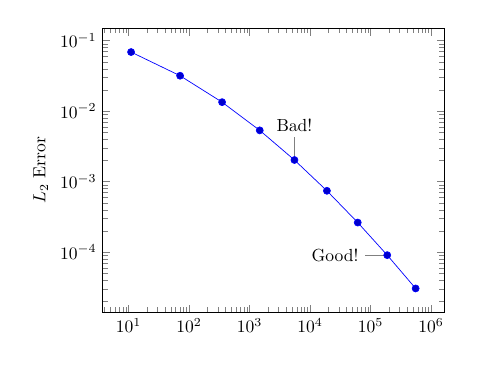
\begin{tikzpicture}[scale = 0.63276]
			\begin{loglogaxis}[
				%xlabel={\textsc{Dof}},
				ylabel={$L_2$ Error},
				]
				\addplot coordinates {
					(11, 6.887e-02)
					(71, 3.177e-02)
					(351, 1.341e-02)
					(1471, 5.334e-03)
					(5503, 2.027e-03)
					(18943, 7.415e-04)
					(61183, 2.628e-04)
					(187903, 9.063e-05)
					(553983, 3.053e-05)
				};
				\node [coordinate,pin=above:{Bad!}]
				at (axis cs:5503,2.027e-03) {};
				\node [coordinate,pin=left:{Good!}]
				at (axis cs:187903,9.063e-05) {};
			\end{loglogaxis}
		\end{tikzpicture}
		\caption{A subfigure}
		\label{fig:sub1}
	\end{subfigure}
	\hfill
	\begin{subfigure}{.49\textwidth}
		\centering
		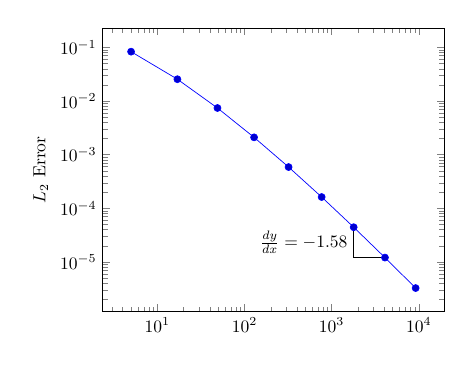
\begin{tikzpicture}[scale = 0.63276]
			\begin{loglogaxis}[
				ylabel=$L_2$ Error,
				]
				\draw
				(1793,4.442e-05)
				|- (4097,1.207e-05)
				node [near start,left]
				{$\frac{dy}{dx} = -1.58$};
				\addplot coordinates {
					(5, 8.312e-02)
					(17, 2.547e-02)
					(49, 7.407e-03)
					(129, 2.102e-03)
					(321, 5.874e-04)
					(769, 1.623e-04)
					(1793, 4.442e-05)
					(4097, 1.207e-05)
					(9217, 3.261e-06)
				};
			\end{loglogaxis}
		\end{tikzpicture}
		\caption{A subfigure}
	  	\label{fig:sub2}
	\end{subfigure}\\

	\begin{subfigure}{.49\textwidth}
		\centering
		\includegraphics[width=.5\linewidth]{\resourcePath eg05}
		\caption{A subfigure}
		\label{fig:sub3}
	\end{subfigure}
	\begin{subfigure}{.49\textwidth}
		\centering
		\includegraphics[width=.5\linewidth]{\resourcePath eg06}
		\caption{A subfigure}
		\label{fig:sub4}
	\end{subfigure}
	\caption{A figure with two subfigures}
	\label{fig:sub}
\end{figure}
 
上靣示例中,子圖\ref{fig:sub1}、子圖\ref{fig:sub2}、子圖\ref{fig:sub3}、子圖\ref{fig:sub4}分別表示子圖








\subsubsection{文獻引用}
 \cite{wangzhenwu2004, wenzaowai2009, qiuziheng2017, hedingzhao2019, qiujiongyou2014b, qiujiongyou9999, linjing2018, linwenyao2018, linxhui2014, chenyaning9999, luey2013, wendamao2015, qiujiongyou2014a, abdoh2019, bordwell2013, bourdieu1990, cole1992, harvey2007, johnson2018, macdonald2020, manguel2009b, milliot9999, poff2019, villazón2011, manguel2009a}
 
\chapter{數學公式}
\begin{equation}
\label{eq1}
e^{\pi i}+1=0
\end{equation}
\begin{align}
2 y & =d\label{eq:IntoSection}\\
3 y & =cx+d\\
4 y_{12} & =bx^{2}+cx+d\\
5 y(x) & =ax^{3}+bx^{2}+cx+d
6 
\end{align}
\begin{equation}
2 x=\left\{ \begin{array}{cl}
3 0 & \textrm{if }A=\ldots\\
4 1 & \textrm{if }B=\ldots\\
5 x & \textrm{this run  text.}\end
{array}\right.
\end{equation}       

 
有門有系統地討論此一問題者為Jensen,在1988 年Jensen 首度有系統地我
收錄以公司治理為主題的文章(Weston, Siu \& Johnson; 2002)。

美國學者對公司治理的討論可追溯自1930 年代,Berle \&
Means(1932)指出,美國企業存在著股權分散的必要性,因為隨著企
業規模不斷的擴大,使得多數的中大型公司皆需將經營權與所有權
加以分離來經營,以期達到專業化的目的。
有系統地討論此一問題者為Jensen,在1988 年Jensen 首度有系統地
收錄以公司治理為主題的文章(Weston, Siu \& Johnson; 2002)。




\subsection{算法表}
\begin{algorithm}[H]
    \fz[10][0.25]
	\SetAlgoVlined %設置帶水平線的連線
	\PrintSemicolon
	\KwData{document set $D :=\{d_1,d_2,\cdots,d_i\}$, term vector $d_1 =\{t_1,t_2,\cdots,t_j\}$
	}
	\KwResult{top6000,High TF-IDF Frequency Keywords}
	\Begin{
	term matrix:$\ \mathcal{L};  \hfill /* \textit{Initial value is empty ($j \times i$)} */$\\
	counter:$\ i =0, j=0;$\\
	    \For{$d  \in D$}{
	        $ i\ $++;\\ 
	        \For {$t \in d$} {
	                $ j\ $ ++;\\[-2mm]
	                $ w_{i,j} = \text{tf}(t,d)\cdot \text{idf}(t,D) = \dfrac{f_{t,d}}{n_d} \cdot \log \dfrac{N}{|\{d \in D: t \in d\}|};$\\
	                $ \mathcal{L}_{i,j}$.Append($t,w_{i,j}$);\\
	            }
            $\mathcal{L}_{i,j}$.Sort(by:$w_{i,j}$)[:10];   \hfill /* \textit{descending rank and retain the top 10.}*/\\
            $\mathcal{L}_{i,j}$.Reindex(); \hfill /* \textit{reset the index.}*/
	        }
   \vspace{-1.5mm} term matrix: $\mathcal{L}= 
    \left[\begin{array}{llll}
    t'_{1,1} & t'_{1,2} & \cdots & t'_{1,10}  \\[-2mm]
    \vdots &\vdots &\vdots & \vdots\\[-1mm]
    t'_{j,1} & t'_{j,2} & \cdots & t'_{j,10}  \\[-1mm]
    \end{array}\right]
    $    \hfill /* \textit{print $\mathcal{L} \ (10\times j)$  result} */\\[0.5em]
    \nlset{Note$^\star$ \ \ \ \ \  }   \textbf{OutputFile: \textbf{File}$^{(1,\divideontimes)}$ } \\[0.5em] 
    \For {$ t' \in \mathcal{L}  $}{
    $i,j \leftarrow t'$ .index()\\[-1mm]
        $w_{i,j} = \text{tf}(t', \mathcal{L}  ) =  \dfrac{f_{t'} }{10 \cdot j} ;$           \hfill /* \textit{where $f_{t'}$ is the raw count of a term $t'$ in $\mathcal{L} $ }*/ \\
    }
     \nlset{Remark$^\star$ \ \ \ \ \  }  $\mathcal{L} $.Sort(by:$w_{i,j}$)[:6000];   \hfill /* \textit{descending rank and retain the top 6000.}*/\\[0.5em]
         \nlset{Note$^\star$ \ \ \ \ \  }   \textbf{OutputFile: \textbf{File}$^{(2,\divideontimes)}$ }  \\[0.5em]
    \textbf{End}
    }	
	\caption{Text Mining: Keyword Extraction Algorithm}
\end{algorithm}

 











% 請確保bib 文件名稱為 ref.bib, 利用js文件處理後的bbl文件名稱為 ref.bbl
\addreference


% 
    \begin{thebibliography}{}

    \bibitem[zh, 2019]{zh2019}{\fontsize{16pt}{\baselineskip}\selectfont{\it\bfseries 中文文獻}}

    \bibitem[方氏等人, 2011]{inbook3}
方氏、方氏、作者二、作者三(2011)。
\newblock  載於楊先生(主編),\textbf{一本書里的一部分內容}(頁 233-666)。楊先生: 中國社會科學出版社。

\bibitem[伍氏, 2011]{manual1}
伍氏(2011)。
\newblock 科技文檔題目。

\bibitem[online22, 无日期]{online22}
李氏(无日期)【GitHub】。澳門科技大學博士論文\LaTeX 模版,沒有日期信息。取自 https://github.com/iihciyekub/MUST-Thesis

\bibitem[online44, 2019年5月29日]{online44}
李氏(2019年5月29日)【GitHub】。澳門科技大學博士論文\LaTeX 模版,有作者與日期信息。取自 https://github.com/iihciyekub/MUST-Thesis

\bibitem[李氏, 2012]{mastersthesis1}
李氏 (2012)。
\newblock \textbf{碩士畢業論文題目}。碩士論文,澳門科技大學。

\bibitem[吳氏等人, 2011]{booklet34}
吳氏、吳氏、作者二、作者三(2011)。
\newblock \textbf{ 沒有出版社的書籍書名}。澳門:中國社會科學出版社。

\bibitem[沈氏, 2012]{proceedings11}
沈氏 (2012)。
\newblock 會議論文集。

\bibitem[馬氏等人, 2011]{misc43}
馬氏、作者二、作者三、作者四、作者五、作者六等人(2011)。
\newblock MISC 類型題目。
\newblock \textbf{******學報},\textbf{11}\textbf{(1)},11-19。

\bibitem[陳氏, 2019]{phdthesis3}
陳氏 (2019)。
\newblock \textbf{博士畢業論文題目}。博士論文,澳門科技大學。

\bibitem[孫氏等人, 2011]{manualwew}
孫氏、作者二、作者三、作者四、作者五、作者六等人(2011)。
\newblock manual 技術手冊。
\newblock \textbf{******學報},\textbf{11}\textbf{(1)},11-19。

\bibitem[張者一等人, 2011]{book34}
張者一、張者一、作者二、作者三(2011)。
\newblock \textbf{ 有確定出版社的書籍書名}。澳門:iihciyekub出版社。

\bibitem[楊氏等人, 2012]{inproceedings22}
楊氏、楊氏、作者二、作者三 (2012)。
\newblock 會議論文集中的一篇文章。

\bibitem[蔡氏等人, 2011]{article32}
蔡氏、作者二、作者三、作者四、作者五、作者六等人(2011)。
\newblock article 類型題目。
\newblock \textbf{******學報},\textbf{11}\textbf{(1)},11-19。

\bibitem[歐陽氏, 2012]{thesis2}
歐陽氏 (2012)。
\newblock \textbf{畢業論文題目}。論文,澳門科技大學。

\bibitem[online33, 无日期]{online33}
澳門科技大學博士論文\LaTeX 模版,沒有作者與日期信息。(无日期)。取自 https://github.com/iihciyekub/MUST-Thesis

\bibitem[online11, 2011年11月09日]{online11}
澳門科技大學博士論文\LaTeX 模版,沒有作者信息。(2011年11月09日)。取自 https://github.com/iihciyekub/MUST-Thesis

\bibitem[En, 2019]{en2019}{\fontsize{16pt}{\baselineskip}\selectfont{\it\bfseries 英文文獻}}

    \bibitem[online3e4, 2011,September 11]{online3e4}
\iiname(2011,September 11)[code resources].A \LaTeX Template For MUST Thesis without author \& data info, Retrieved from https://github.com/iihciyekub/MUST-Thesis

\bibitem[online2e2, n.d.]{online2e2}
\iiname(n.d.)[GitHub].A \LaTeX Template For MUST Thesis without data info, Retrieved from https://github.com/iihciyekub/MUST-Thesis

\bibitem[online1e1, 2011,September 11]{online1e1}
A \LaTeX Template For MUST Thesis without author info,(2011,September 11), Retrieved from https://github.com/iihciyekub/MUST-Thesis

\bibitem[Alisa \& David, 2012]{mastersthesis}
Alisa (2012).
\newblock {\em Mastersthesistitle}. Master dissertation,  mac of Technology.

\bibitem[online3e3, n.d.]{online3e3}
A \LaTeX Template For MUST Thesis without author \& data info,(n.d.), Retrieved from https://github.com/iihciyekub/MUST-Thesis

\bibitem[Fundel, 2007]{thesis}
Fundel,K. (2007).
\newblock {\em Text mining and gene expression analysis towards combined interpretation of high throughput data}. Dissertation, lmu.

\bibitem[Ignatow \& Mihalcea, 2016]{book1}
Ignatow,G. (2016).
\newblock {\em Text mining: a guidebook for the social sciences}. Sage Publications.

\bibitem[Kongthon, 2004]{phdthesis}
Kongthon,A. (2004).
\newblock {\em A text mining framework for discovering technological intelligence to support science and technology management}. Doctoral dissertation, Georgia Institute of Technology.

\bibitem[Larsen \& Aone, 2011]{inbook}
Larsen,B. (2011).
\newblock  Semantic analysis. In Kongthon (Ed.), {\em Machine learning wtih something} (pp. 233-666). Kongthon: Acm Computing Surveys.

\bibitem[Macedo et al., 2009]{inproceedings}
Macedo,A.L., Reategui,E., Lorenzatti,A., \& Behar,P. (2009).
\newblock Using text-mining to support the evaluation of texts produced collaboratively. Springer (pp. 368--377).

\bibitem[Sebastiani et al., 1988]{misc2}
Sebastiani,F.S.G., Buckley,C., Buckley,C.S.G., Buckley,C., Buckley,C., Buckley,C., et al (1988).
\newblock Term-weighting approaches in automatic text retrieval.
\newblock {\em Information Processing \& Management}, 513-523.

\bibitem[Null, 2012]{manual}
Null (2012).
\newblock Technology manual.

\bibitem[Teahan \& Harper, 2001]{proceedings}
Teahan,W.J. (2001).
\newblock Combining ppm models using a text mining approach. IEEE (pp. 153--162).

\bibitem[Talton et al., 2011]{booklet}
Talton,H., Buckley,W., \& Yue,R. (2011).
\newblock {\em Machine learning in automated text categorization}. Beijing:Acm Computing Surveys.

\bibitem[Vickman, 2007]{article1}
Vickman,T.A. (2007).
\newblock The changing digital dynamics of multichannel marketing the feasibility of the weblog: text mining approach for fast fashion trending.
\newblock {\em Journal of Fashion Marketing and Management}, {\em 11}(4), 604-+.

\end{thebibliography}
    











\begin{appendix}
證明過程
\end{appendix}











\begin{acknowpage}
謝謝各位
\end{acknowpage}









 
\begin{addcvpage}
% 設置門入學時間 
\addedudate{2019 年 7 月}




% 填寫教育經歷,注意內容以逗號作分隔,
\addeduItem{2009.16-2012.13,中國澳門氹仔島澳門科技大學,商學院}
\addeduItem{2009.16-2012.13,澳門科技大學,商學院}
\addeduItem{2009.16-2012.13,澳門科技大學,商學院}



%增加學術文章
\addpaperItem{ 
    \item 中國澳門氹仔島澳門科技大學1中國澳門氹仔島澳門科技大學1中國澳門氹仔島澳門科技大學1中國澳門氹仔島澳門科技大學1中國澳門氹仔島澳門科技大學1中國澳門氹仔島澳門科技大學1中國澳門氹仔島澳門科技大學1中國澳門氹仔島澳門科技大學,
    \item 中國澳門氹仔島澳門科技大學,
}




% 增加項目
\addprojectItem{
    \item 中國澳門氹仔島澳門科技大學,商學院商學院
    \item  商學院商學院商學院中國澳門氹仔島澳門科技大學,商學院商學院商學院商學院商學院中國澳門氹仔島澳門科技大學,商學院商學院商學院商學院商學院 
}
\end{addcvpage}









\end{document}
